%
% main.tex -- Paper zum Thema <elektro>
%
% (c) 2020 Autor, OST Ostschweizer Fachhochschule
%
% !TEX root = ../../buch.tex
% !TEX encoding = UTF-8
%
\chapter{Zweidimensionale Elektrostatik 
\label{chapter:elektro}}
\kopflinks{Thema}
\begin{refsection}
\chapterauthor{Malenka Hossli und Andrea Studer}

%
% einleitung.tex -- Beispiel-File für die Einleitung
%
% (c) 2020 Prof Dr Andreas Müller, Hochschule Rapperswil
%
% !TEX root = ../../buch.tex
% !TEX encoding = UTF-8
%

\section{Einleitung}
Elektrostatik wird für uns Menschen primär dann erfahrbar, wenn es im Vorfeld zur Ladungstrennung gekommen ist.
Blitze, Van de Graaff Bandgeneratoren, klebende Styroporkügelchen --- Grundlage für diese physikalischen Ereignisse ist folgendes Prinzip:
Gleichartige Ladungen stossen sich ab, ungleichartige Ladungen ziehen sich an.
So kann es passieren, dass wir einen synthetischen Pullover über den Kopf ziehen, ein Knistern hören, und sobald wir dann einen anderen (geerdeten) Menschen berühren, funkt es.
Dieses kurze Zwicken beweist die unsichtbare elektrostatische Aufladung, die durch Reibung des Pullovers erzeugt worden ist.
Als Fachpersonen im Bereich der Elektrotechnik haben wir häufig Bauteilchen in der Hand, die wir vor elektrostatischer Entladung (ESD) schützen müssen, da diese Chips oder ICs (Integrated Circuits) schon durch kleine Ladungsspitzen zerstört werden können.
Zum Schutz empfindlicher Bauteile tragen wir daher geerdete Armbänder, was Ladungstrennung, welche zu ESD führt, verhindert. 

Um elektrostatische Aufladung zu demonstrieren, wird die (langhaarige) Versuchsperson daher zuallererst auf ein isoliertes Podest gestellt.
Ladung, die durch den von Robert Van de Graaff 1929 erfundenen Generator auf eine Metallkugel gebracht wird, gelangt mittels Berührung der Handflächen auf die Versuchsperson.
\textcolor{red}{TODO Foto Versuchsperson mit Feldlinien eingezeichnet}
Der Van de Graaff Generator nutzt die mechanische Reibung eines Gummibandes, um gleichartige Ladungsträger auf einer Metallkugel abzuladen, welche sich anschliessend durch Influenz auf der ganzen Oberfläche verteilen.
Es spielt dabei keine Rolle, ob die Ladungsträger positiv oder negativ sind.
Die Ladungen wandern auf die Versuchsperson, und da sie sich abstossen entsteht eine kleine Kraft.
Diese reicht bei genügend trockener Luft aus, um die Haare der Versuchsperson zu Berge stehen zu lassen.
Trotz seines tiefen Wirkungsgrades kommt der Van de Graaff Generator zur Erzeugung hoher Gleichspannungen als Teilchenbeschleuniger zum Einsatz \cite{elektro:lexikon}.

In diesem Paper wird zweidimensionale Elektrostatik durch das Werkzeug Geometrie sichtbar gemacht.
Die Reduktion auf zwei Dimensionen führt dazu, dass von den vier Maxwell-Gleichungen nur noch eine relevant ist, nämlich die Laplace Gleichung für das Potential. 
Diese Gleichung wird hergeleitet und genauer erklärt.
Der Fokus liegt auf dem Zusammenhang zwischen elektrischen Feldlinien und Äquipotentiallinien im zweidimensionalen Raum.
Feldlinien und Potential werden als komplexe Funktionen interpretiert und über komplexe Abbildungen miteinander verknüpft.
Wie das funktioniert, wird anhand von vielen Beispielen in diesem Kapitel erklärt, bewiesen und veranschaulicht. 



\section{Grundlagen der Elektrostatik\label{elektro:section:EFeld}}
\kopfrechts{Grundlagen der Elektrostatik}

Elektrostatik ist die Lehre von ruhenden elektrischen Ladungen und deren Wirkung auf ihre Umgebung, insbesondere andere Ladungen und Materie \cite{elektro:elt2_skript}.
Es fliesst kein elektrischer Strom und in der Folge gibt es keinen Widerstand. 
Elektrostatische Grössen besitzen keine zeitliche Abhängigkeit.
Mathematisch formuliert: Die erste Ableitung nach der Zeit ist für alle elektrostatischen Funktionen gleich Null: $\frac{\partial \vec{E}}{\partial t} = 0$.

\subsection{Vektor- und Skalarfeld, Quellenfeld und Homogenität
\label{elektro:subsection:VektorSkalar}}
Das elektrische Feld ist ein Vektorfeld.
Das bedeutet, jedem Punkt im Raum wird ein Betrag und eine Richtung der elektrischen Feldstärke zugeordnet. 
Das Potentialfeld ist ein Skalarfeld.
Jedem Punkt im Raum wird der Betrag des Potentials in Volt zugeordnet, aber keine Richtung.

Elektrostatische Felder sind Quellenfelder.
Sie sind statisch, also nicht dynamisch, und stehen im Gegensatz zu Wirbelfeldern, welche beispielsweise durch sich zeitlich ändernde Magnetfelder erzeugt werden können.
Die Feldlinien des elektrostatischen Felds beginnen immer auf positiven Ladungen und enden auf negativen. 
Die Ladung kann sich dabei auch im Unendlichen befinden.
TODO: Bild einfügen.

Verlaufen die Feldlinien parallel, spricht man von einem homogenen Feld, ansonsten von einem inhomogenen Feld.
Das Feld zwischen zwei parallelen Kondensatorplatten beispielsweise ist homogen, was die mathematische Berechnung erheblich erleichtert. 

\subsection{Das Coulomb-Gesetz
\label{elektro:subsection:Coulomb}}
Das Coulomb-Gesetz beschreibt die Kraft zwischen zwei ruhenden Punktladungen.
Eine Punktladung ist per Definition eine punktsymmetrische Ladung ohne  räumliche Ausdehnung.
In der Praxis ist das Coulomb-Gesetz für reale geladene Körper in guter Näherung gültig.
Insbesondere, wenn der Abstand zwischen den geladenen Körpern viel grösser ist als die Körper selbst.

\begin{equation}
	\vec{F} = \frac{Q_1 Q_2}{4\pi\varepsilon_0 R^{2}}\hat{R}
    \label{equation:Coulomb}
\end{equation}

Die Coulomb-Kraft nimmt mit dem Produkt der Ladungen $Q_1$ und $Q_2$ zu und mit dem Quadrat des Abstands $R$ zwischen den Ladungen ab.
$\vec{R} = R \cdot \hat{R}$ ist der Distanzvektor zwischen den Ladungen und zeigt vom Ort der Ursache auf den Ort der Wirkung.
$\hat{R}$ ist in der Elektrotechnik der Einheitsvektor mit Richtung von $\vec{R}$.
Liegt einer der Punkte im Ursprung wird die Variable $r$ verwendet.
Die beiden Komponenten des Vektors sind der Betrag $R$ und die Richtung $\hat{R}$, diese werden in der Formel \eqref{equation:Coulomb} separat verwendet.
Das Coulomb-Gesetz gilt für Distanzen zwischen $10^{-16}$ und $10^{8}$ Metern. 
Für $R = 0$ ist es nicht definiert. 
$\varepsilon_0$ ist die elektrische Permittivität des Vakuums und beträgt ungefähr 8.854 pF/m. 

\subsection{Das elektrische Feld}
Das elektrische Feld und die Coulomb-Kraft sind definitionsgemäss eng verwandt.
Bringt man eine Probeladung $q$ in die Nähe einer Punktladung $Q$, so ist die Kraft, welche auf die Probeladung wirkt, als elektrische Feldstärke definiert.
Sie ist das gesamte vektorielle Kraftfeld, das an der jeweiligen Stelle auf $q$ wirkt, und wird in Volt pro Meter angegeben.
Es handelt sich um ein Radialfeld (ausgehend von der positiven oder führend zur negativen Quelle).
\begin{equation}
	\vec{E} = \frac{\vec{F}}{q} = \frac{\text{Kraft}}{\text{Probeladung}} = \frac{Q}{4\pi\varepsilon_0 r^{2}}\hat{r}
    \label{equation:EFeld}
\end{equation}


\subsection{Das elektrische Potential $\varphi$
\label{elektro:subsection:Potential}}
Genau wie beim $\vec{E}$-Feld, das durch Normalisierung der Coulomb-Kraft mit einer Probeladung definiert wird, ist das elektrische Potential durch Normalisierung der Energie $W$ mit einer Probeladung definiert.
\begin{equation}
	\varphi = \frac{W}{q} = \frac{Q}{4\pi\varepsilon_0r} = - \int_{\text{Ref}}^P \vec{E} \cdot d\vec{l}
    \label{equation:Potential}
\end{equation}
Die Einheit von $\varphi$ ist Volt, genau wie bei der Spannung, denn die Spannung ist nichts anderes als die Differenz zweier Potentiale.
Im Gegensatz zum elektrischen Feld, welches ein Vektorfeld ist, ist das Potentialfeld ein Skalarfeld.
Die Potentiale jedes einzelnen Punktes ergeben einen Gradienten, aus dem die elektrische Feldstärke berechnet werden kann.
Das negative Vorzeichen in der Formel \eqref{equation:Potential} hat seinen Ursprung in der Wahl des Bezugssystem, der Referenz Ref, von wo aus integriert wird.


\subsection{Äquipotentiallinien
\label{elektro:subsection:Aequipotentiallinien}}
Orte, die dasselbe Potential aufweisen, also äquipotential sind, nennt man im zweidimensionalen Raum Äquipotentiallinien.
Auf diesen Linien kann eine Probeladung beliebig verschoben werden, ohne dass dabei Arbeit aufgewandt werden muss.
Äquipotentiallinien liegen stets senkrecht zum elektrischen Feld.

\subsection{Beispiel Einheitskreis
	\label{elektro:subsection:Einheitskreis-Beispiel}}
Zeichnet man im elektrostatischen Radialfeld einer positiven oder negativen Punktladung die Äquipotentiallinien ein, resultieren Kreise mit unterschiedlichen Radien.
Es erscheint intuitiv, dass man bei bekanntem $\vec{E}$-Feld die Äquipotentiallinien sofort einzeichnen kann, was in diesem Beispiel besonders einfach ist.
Umgekehrt funktioniert es aber auch: Dazu werden komplexe Funktionen und konforme Abbildungen verwendet.

\section{Komplexe Funktionen in der Elektrostatik
\label{elektro:section:Funktionen-komplexer-Var}}
Zur Erinnerung: Eine komplexe Zahl $z$ wird in kartesischen Koordinaten als Real- und Imaginärteil wie folgt dargestellt: $z = x + iy$.
Eine komplexe Funktion $f(z) = u + iv$ kann aufgeteilt werden in zwei Funktionen $u = u(x,y)$ und $v = v(x,y)$, die von den realen Variablen $x$ und $y$ abhängig sind.
Ein erstes Beispiel ist die Funktion $f(z) = z^{2}$.
Da mit den Real- und Imaginärteilen wie gewohnt gerechnet werden kann, ergibt das Quadrieren: 
\begin{equation}
	(x+iy)^{2} = x^{2} - y^{2} + i2xy,
\end{equation} 
mit
\begin{equation}
	u(x,y) = x^{2} - y^{2}
\end{equation} 
und 
\begin{equation}
	v(x,y) = 2xy.
\end{equation}

\subsection{Holomorphe oder analytische Funktion
\label{elektro:subsection:holomorph}}
Die kontinuierlichen Funktionen $u(x,y)$ und $v(x,y)$ mit kontinuierlichen partiellen Ableitungen sind dann holomorph, wenn sie die Cauchy-Riemann Gleichungen
\begin{equation}
	\label{elektro:subsection:holomorph:Cauchy1}
	\frac{\partial u}{\partial x} = \frac{\partial v}{\partial y}
\end{equation}
und 
\begin{equation}
\label{elektro:subsection:holomorph:Cauchy2}
	\frac{\partial u}{\partial y} =
	- \frac{\partial v}{\partial x}
\end{equation}

erfüllen.
Holomorph bedeutet differenzierbar in jeder Ordnung und darstellbar als Exponentialreihe.
Das Integral der Funktion entlang eines geschlossenen Weges in der komplexen Zahlenebene ist Null
\begin{equation}
	\oint f(z) \,dz = 0.
\end{equation}
\textcolor{red}{Streichen, auf Kapitel 1 und 2 verweisen}

\subsection{Laplace Gleichung
	\label{elektro:subsection:Laplace}}
Leitet man die beiden Cauchy-Riemann Gleichungen \eqref{elektro:subsection:holomorph:Cauchy1} und \eqref{elektro:subsection:holomorph:Cauchy2} noch einmal ab nach x und y und addiert bzw. subtrahiert die Ergebnisse, dann resultieren
\begin{equation}
	\frac{\partial^{2}u}{\partial x^{2}} + \frac{\partial^{2}u}{\partial y^{2}} = 0
\end{equation}
und 
\begin{equation}
	\frac{\partial^{2}v}{\partial x^{2}} + \frac{\partial^{2}v}{\partial y^{2}} = 0.
\end{equation}
Demzufolge erfüllen die Funktionen $u(x,y)$ und $v(x,y)$ die Laplace Gleichungen
\begin{equation}
	\Delta u = 0
\end{equation}
und 
\begin{equation}
	\Delta v = 0.
\end{equation}
Wenn eine der beiden Funktionen $u$ oder $v$ bekannt ist, kann die jeweils andere Funktion bestimmt werden.
Wenn $u$ bekannt ist, können wir schreiben:
\begin{equation}
	dv = \frac{\partial v}{\partial x}dx + \frac{\partial v}{\partial y} dy = 
	-\frac{\partial u}{\partial y}dx + \frac{\partial u}{\partial x}dy
\end{equation}
und diese Gleichung integrieren, um v zu bestimmen.

Die beiden Vektoren
\begin{equation}
	\nabla{u} = \left(\frac{\partial u}{\partial x}, \frac{\partial u}{\partial y} \right)
\end{equation}
und 
\begin{equation}
	\nabla{v} = \left(\frac{\partial v}{\partial x}, \frac{\partial v}{\partial y} \right)
\end{equation}
stehen senkrecht aufeinander, das heisst sie sind normal zu einander:
\begin{equation}
	\vec{u} \cdot \vec{v} = 0.
\end{equation}
Das bedeutet, die beiden Funktionen $u(x,y)$ und $v(x,y)$ sind lokal senkrecht in ihren Schnittpunkten.

\subsection{Konforme Abbildung
	\label{elektro:subsection:KonformeAbb}}
Eine Abbildung eines Gebietes der komplexen Ebene 1 in ein Gebiet der komplexen Ebene 2 mittels einer komplexwertigen Funktion $f(z)$ heisst konforme Abbildung, wenn die Schnittwinkel zweier beliebiger Kurven der Grösse nach erhalten bleiben. Die durch eine analytische Funktion f(z) erzeugte Abbildung ist für alle Punkte z konform, für die die erste Ableitung nicht verschwindet \cite{elektro:mathematik-alpha}.

%\subsection{Gausssches Gesetz
%\label{elektro:subsection:Gauss}}



%\subsection{Zusammenhang zwischen E-Feld und Potential
%\label{elektro:subsection:ephizusammenhang}}
%Etwas vorgreifend wird hier gezeigt, wie im Falle eines Kreises mathematisch von einem Potentialfeld $\varphi$ auf das elektrische Feld $\mathbf{E}$ geschlossen werden kann.
%Die Fläche außerhalb des Kreises wird als Potentialfeld beschrieben.

%
% teil1.tex -- Beispiel-File für das Paper
%
% (c) 2020 Prof Dr Andreas Müller, Hochschule Rapperswil
%
% !TEX root = ../../buch.tex
% !TEX encoding = UTF-8
%


\section{Riemannscher Abbildungssatz
\label{elektro:section:RiemannSatz}}
\kopfrechts{Riemannscher Abbildungssatz}

Georg Fridrich Bernhard Riemann (1826-1866) \cite{elektro:riemann} war ein deutscher Mathematiker, der sich mit diversen Gebieten der Mathematik beschäftigte.
Auf vielen hat er bahnbrechende Ergebnisse erzielt, die bis heute von grosser Bedeutung sind.
Auch Einstein hat von seinen Theorien Gebrauch gemacht.
Den riemannschen Abbildungssatz hat er erstmals als Skizze im Jahre 1851 in seiner Dissertation veröffentlicht. 
Erst später wurde dieser Satz von anderen Mathematikern formal bewiesen und in die Mathematik eingeführt. 
Es wurden verschiedene Beweise für den riemannschen Abbildungssatz gefunden, die alle auf unterschiedlichen mathematischen Gebieten basieren.
Hier wird der verbreitetste Beweis vorgestellt, der auf dem Satz von Montel basiert, welcher die Existenz konformer Abbildungen auf einfach zusammenhängende Gebiete beschreibt.
Beschreiben ist hier wörtlich gemeint, denn es gibt für den Riemannschen Abbildungssatz keine allgemeine Formel, die für alle Gebiete gilt, sondern nur den Existenzbeweis einer Abbildung.
Das bedeutet, dass für jegliche Figuren eine Transformation existiert.
Diese muss aber auf anderem Weg ermittelt werden, dazu mehr in Abschnitt \ref{elektro:section:KreisTrafo}.

Im Allgemeinen ist unser Ziel ein Gebiet $G$ auf ein einfacheres Gebiet $G'$ abzubilden, um die Berechnung von Potentialfeldern und elektrischen Feldern zu vereinfachen. 
Das Zielgebiet $G'$ ist für uns der Einheitskreis, dessen Potentialfeld $\varphi$ und dessen elektrisches Feld $\vec{E}$ aus Abschnitt \ref{elektro:subsection:Einheitskreis-Beispiel} bereits bekannt sind.

\subsection{Voraussetzungen
\label{elektro:subsection:RiemannVoraussetzungen}}
Zunächst müssen ein paar Voraussetzungen für den riemannschen Abbildungssatz erfüllt sein, damit der Satz überhaupt angewendet werden kann:

\subsubsection{Einfach zusammenhängende Gebiete}
Das ursprüngliche Gebiet $G$ muss einfach zusammenhängend sein, das bedeutet, dass es keine Löcher in dem Gebiet gibt. 
Das Gebiet $G$ darf beliebig gross und beliebig geformt sein, solange es keine ausgeschnittenen Bereiche enthält.
Zu dieser Definition gehört auch, dass das Gebiet offen sein muss. 
Der Rand des Gebiets gehört demzufolge nicht zum Gebiet dazu.
Da sich meistens herausstellt, dass der Rand sich $\grqq$brav$\grqq$ mit verformt und die Abbildung auf dem Rand ebenfalls konform ist, wird in den nachfolgenden Beispielen stets angenommen, dass der Rand analog zur Fläche verformt wird.

%1. Pull Request Version
%Der Rand müsste separat betrachtet werden, wobei sich meistens herausstellt, dass dieser sich $\grqq$brav$\grqq$ mit verformt und die Abbildung auf dem Rand ebenfalls konform ist.
%Es entstehen erst dann Abweichungen, wenn der Rand ausgefallene Fraktale bildet.
%Dies ist in diesen Beispielen nicht der Fall, daher wird stets angenommen, dass der Rand analog zur Fläche verformt wird.

\subsubsection{Teilgebiete der komplexen Ebene}
$ G \subset \mathbb{C} $ muss gelten, dies bedeutet, dass $G$ eine Teilmenge von $\mathbb{C}$ ist.
Für die ganze komplexe Ebene gilt der riemannsche Abbildungssatz.
Würde die gesamte komplexe Ebene auf den Einheitskreis abgebildet werden, dann müssten Punkte, die bereits im Innern des Einheitskreises liegen, unberührt bleiben und jene, welche ausserhalb liegen, müssten auf bereits besetzte Punkte transformiert werden. 
Dies stünde im Widerspruch zur nächsten Voraussetzung, nämlich der Bijektivität der Abbildung.

\subsubsection{Bijektive Abbildung}
Eine bijektive Abbildung ist sowohl injektiv (verschiedene Elemente der Definitionsmenge werden auf verschiedene Elemente der Zielmenge abgebildet) als auch surjektiv (jedes Element der Zielmenge wird getroffen).
Es gibt keine zwei Punkte, welche auf denselben Zielpunkt abgebildet werden. 
Bei der Transformation und auch bei der Rücktransformation geht keine Information verloren und die Abbildung ist umkehrbar.

% \subsection{Existenzbeweis
% \label{elektro:subsection:Riemannbeweis}}
% Im Folgenden wird der Existenzbeweis für den Riemannschen Abbildungssatz vorgestellt in einer Version die auf grundlegenden Eigenschaften von holomorphen Funktionen basiert.
% Er macht sich den Satz von Montel und den Satz von Hurwitz zu Nutze. 

% Es sei $z_0 \in G$ gewählt, $G$ ist dabei das einfach zusammenhängende Gebiet, dass alle voraussetzen wie in Abschnitt \ref{elektro:subsection:RiemannVoraussetzungen} beschrieben erfüllt.
% Es werden nun alle holomorphen Funktionen $f$ betrachtet, die $G$ auf die Einheitskreisscheibe $\mathbb{D}$ abbilden und dabei die Bedingung $f(z_0) = 0$ erfüllen.
% Dann wird die Funktion gesucht für die $\vert f(z_0) \vert '$ maximal ist, damit haben wir ein Maximierungsproblem formuliert, dass es zu lösen gilt.

% \subsubsection{Funktionsklasse
% \label{elektro:subsubsection:RiemannFunktionsklasse}}
% Die holomorphen Funktionen bilden eine Funktionsklasse, die wir mit $\mathcal{F}$ bezeichnen.
% Es muss nun gezeigt werden, dass diese Klasse nicht leer sein kann. 
% Dazu wird ein weiterer Punkt definiert der ausserhalb des Gebiets $G$ liegt der als Abbildungspunkt für $z$ dient.
% Das $a \notin G$ gewählt wird, ist dabei wichtig, da sonst die Abbildung nicht bijektiv wäre.
% $z - a \neq 0$ für alle $z \in G$, existiert auf $G$ ein holomorpher Zweig der Quadratwurzel, $g(z)= \sqrt{z-a}$n. \textcolor{red}{Beschreib wie dies zustande kommt.}
% Die Funktion $g(z)$ ist injektiv, $g(z_1) = g(z_2)$ ist impliziert durch $z_1 -a = g(z_2)^2 = z_2 - a$, damit ist klar, das die Wahl der Lösung der Quadratwurzel eindeutig sein wird. \textcolor{red}{evtl. unverständlich}

% \subsubsection{Maximierungsproblem
% \label{elektro:subsubsection:RiemannMax}}
% $M = \sup (\vert f'(z_0) \vert)$ ist die maximale Ableitung der holomorphen Funktion $f$ an der Stelle $z_0$.
% Dafür wird nun eine Folge $(f_n) \in \mathcal{F}$ gesucht, die die Bedingung $\vert f_n'(z_0) \vert \to M$ erfüllt.


\subsection{Existenzbeweis
\label{elektro:subsection:Riemannbeweis}}
Der Existenzbeweis basiert auf dem Satz von Montel und dem Satz von Hurwitz, wobei ein Maximierungsproblem formuliert wird, das es zu lösen gilt.
Es wird hier nur über das Vorgehen berichtet, der Beweis selbst ist zu umfangreich um ihn hier darzustellen. \textcolor{red}{Quelle wo er nachgesehen werden kann}
Gestartet wird damit einen Punkt $z$ innerhalb und einen Punkt $a$ ausserhalb des Gebiets $G$ zu wählen, die als Abbildungspunkte dienen. 
Es gilt $z \in G \land a \neq G$.
Es wird die Distanz $d = \vert z - a \vert$ zwischen den beiden Punkten definiert.
Mit der Quadratwurzelfunktion kann eine holomorphe Funktion (siehe Abschnitt \ref{elektro:subsection:holomorph}) $g(z) = \sqrt{z - a}$ auf dem Gebiet $G$ definiert werden.
Daraus ergibt sich eine Funktionsklasse $\mathcal{F}$, die alle holomorphen Funktionen $f$ enthält, die $G$ auf die Einheitskreisscheibe $\mathbb{D}$ abbilden und dabei die Bedingung $f(z_0) = 0$ erfüllen.
Für den weiteren Beweis werden verschiedene Eigenschaften der holomorphen Funktionen verwendet, wie die Surjektivität, welche die Extremalfunktion aufweisen muss, sowie Automorphien der Einheitskreisscheibe, welche die Abbildung auf den Kreis beschreiben.
Das Ganze läuft darauf hinaus, das gezeigt werden kann das die Abbildungsfunktion $f$ sowie auch die Rücktransformation $f^{-1}$ holomorph sind und damit die Abbildung konform ist. 
Womit der Satz von Riemann bewiesen ist.
%
% teil2.tex -- Beispiel-File für teil2 
%
% (c) 2020 Prof Dr Andreas Müller, Hochschule Rapperswil
%
% !TEX root = ../../buch.tex
% !TEX encoding = UTF-8
%
\section{Der Kreis
\label{elektro:section:DerKreis}}
\kopfrechts{Der Kreis}
Bevor wir im nächsten Kapitel die Transformation von Kreisen betrachten, wollen wir uns mit den Eigenschaften des Kreises beschäftigen.
Der Kreis ist die einfachste und am besten verstandene Figur der Mathematik.
Elektrostatische Feldlinien und auch das Potential können leicht berechnet werden.
Für die elektrostatische Betrachtung dieses Kapitels ist der Kreis optimal, denn sowohl die Formeln für $\vec{E}$ als auch für $\varphi$ hängen nur vom Abstand zum Mittelpunkt $r$ ab.


\subsection{Radialsymmetrische Potentiale
\label{elektro:subsection:RadialsymmetrischePotentiale}}
Im Kreis ist das Potential radialsymmetrisch verteilt.
Der Kreis stellt eine Punktladung mit der Ladungsdichte $\rho$ dar.
%Zur Berechnung des Feldes wird das ... verwendet in seiner Integralform. 
Dank der Punktsymmetrie des Kreises ist das Potentialfeld durch Polarkoordinaten, die den Abstand $r$ und den Winkel $\varphi$ darstellen, vollständig beschrieben.  
Im Abschnitt \ref{elektro:subsection:Einheitskreis-Beispiel} wurde gezeigt wie das Potentialfeld $\varphi$ und das elektrische Feld $\vec{E}$ zusammenhängen.
Es ergibt sich ein Kreislauf von Integralen, in welchem stets von einem Fall auf den anderen geschlossen werden kann und umgekehrt.
Dazu muss jedoch eine dieser Formeln, die für den Kreis gültig ist, aufgestellt worden.
Es braucht also einen Einstieg, durch den die Integralformel des elektrischen Feldes $\vec{E}$ gefunden werden kann. 

\begin{equation}
    \varphi = \int_{-\infty}^{\infty} \frac{\rho}{4\pi\varepsilon_0 r} dV
    \label{elektro:equation:potentialbegin}
\end{equation}
Wie zuvor gezeigt, stellt der Kreis die Ladung dar und wir wollen das Potentialfeld ausserhalb des Kreises beschreiben.
Dazu können wir das Integral von der Kreisoberfläche bis in die Unendlichkeit lösen.
\begin{equation}
    \varphi = \int_{0}^{2\pi} \int_{r}^{\infty} \frac{\rho}{4\pi\varepsilon_0 r} r \, dr \, d\varphi
    = \frac{\rho}{2\varepsilon_0} \int_{r}^{\infty} dr
    = \frac{\rho}{2\varepsilon_0} [r]_{r}^{\infty}
    = -\frac{\rho}{2\varepsilon_0} r
\end{equation}
Die abbildung dieser Formel ist in Abbildung \ref{elektro:figure:phi_feld_kreis} dargestellt.

Verständnis: 
Das Volumenelement wird zu $dV = r \, dr \, d\varphi $.
Für beide Integrale wird die Integrationsgrenze von $0$ bis $2\pi$ für $\varphi$ und von $r$ bis $\infty$ für $r$ gewählt, da das Potentialfeld ausserhalb des Kreises beschrieben werden soll und dies um die gesamten $2\pi$ des Kreises.


\subsection{Kreisspiegelung
\label{elektro:subsection:Kreisspiegelung}}

Damit man sich die Kreisspiegelung vorstellen kann, wird der Kreisrand als Spiegeloberfläche angenommen. 
Somit wird jeder Punkt ausserhalb des Kreises --- auch die Unendlichkeit --- in das Innere des Einheitskreises gespiegelt.
Analog dazu wird alles innerhalb des Einheitskreises nach aussen gespiegelt, wobei der Ursprung auf alle Seiten in die Unendlichkeit gespiegelt wird. 

Diese Transformation wird hier nur gezeigt, weil durch diese Transformation die Wahl der Integralgrenzen im Abschnitt \ref{elektro:subsection:RadialsymmetrischePotentiale} erklärt werden kann.
Es kann vom Mittelpunkt zum Kreisrand oder vom Kreisrand bis in die Unendlichkeit integriert werden und mit einer einfachen Kreisspiegelung im Komplexen vom einen zum anderen Fall übergegangen werden. 
Mathematisch wird die Kreisspiegelung durch die Transformation
\begin{equation}
    z \mapsto \frac{1}{\overline{z}}
\end{equation}
beschrieben.
\textcolor{red}{Kreisspiegelung Fallüberführung rechenbeispiel}


\subsection{Zusammenhang zwischen $\vec{E}$-Feld und Potential
\label{elektro:subsection:ephizusammenhang}}
Anhand des Beispiels des Einheitskreises wird hier gezeigt wie von einem Potentialfeld $\varphi$ auf das elektrische Feld $\vec{E}$ geschlossen werden kann, wie im Abschnitt \ref{elektro:subsection:Einheitskreis-Beispiel} behauptet wird.

Unser Ausgangspunkt ist das elektrische Feld $\vec{E}$, das durch die Umformung zu zylindrischen Koordinaten auf $ \vec{E} = \frac{\rho}{2\pi\varepsilon_0 r} \hat{r} $ vereinfacht werden kann.
Wird dies in die Formel \ref{equation:Potential} eingesetzt, so ergibt sich das Potentialfeld $\varphi$. 
\begin{equation}
    \varphi = - \int_{1}^{k} \frac{\rho}{2\pi\varepsilon_0 r} \hat{r} \cdot d\mathbf{r}
    = - \frac{\rho}{2\pi\varepsilon_0}\vert ln(k) \vert_{1}^{r}
    = - \frac{\rho}{2\pi\varepsilon_0} \operatorname{ln}(r)
    \label{elektro:equation:potential}
\end{equation}
Ist nun das Elektrische Feld bekannt, kann daraus auch das elektrische Potential berechnet werden.
% Kontinuierlich kann auch vom Potentialfeld $\varphi$ auf das elektrische Feld $\mathbf{E}$ geschlossen weerden indem die Formel die sich aus dem soeben ausgeführen Integrals umgestellt wird. 
Der Rückschluss vom Potentialfeld $\varphi$ auf das elektrische Feld $\vec{E}$ ist über die Laplace-Gleichung \ref{elektro:subsection:Laplace} möglich.
Es muss konsistent in zylindrischen Koordinaten gearbeitet werden, damit die Ableitung des Potentials $\varphi$ nach $r$ das elektrische Feld $\vec{E}$ ergibt.

\begin{equation}
    \vec{E} = - \nabla \varphi = - \frac{\partial}{\partial r} \left( - \frac{\rho}{2\pi\varepsilon_0} \operatorname{ln}(r) \right) = \frac{\rho}{2\pi\varepsilon_0 r} \hat{r}
    \label{elektro:equation:efeld}
\end{equation}

Hiermit ist gezeigt, dass die Integrale in einem Kreislauf miteinander verbunden sind und von einem zum anderen geschlossen werden kann.

\subsubsection{Komplexe Darstellung}
Die formeln können nun noch für Komplexe Zahlen tauglich gemacht werden indem der Vektor $\vec{r}$ in Kartesisschen Koordinaten dargestellt wird und danach die Feldanteile Komplex geschrieben werden.
//TODO: nochmals drübergehen bezüglich der Schreibweise und der Herleitung.

\begin{equation}
\begin{aligned}
    \vec{E}
    &=
    \frac{\rho}{2\pi\varepsilon_0 r}\hat{r}
    \\[2mm]
    &=
    \frac{\rho}{2\pi\varepsilon_0 r}
    \left(
    \frac{x}{r}\hat{x}
    +
    \frac{y}{r}\hat{y}
    \right)
    \\[2mm]
    &=
    \frac{\rho}{2\pi\varepsilon_0}
    \left(
    \frac{x}{r^2}\hat{x}
    +
    \frac{y}{r^2}\hat{y}
    \right)
    \\[2mm]
    &=
    \frac{\rho}{2\pi\varepsilon_0}
    \left(
    \frac{x}{x^2+y^2}\hat{x}
    +
    \frac{y}{x^2+y^2}\hat{y}
    \right).
\end{aligned}
\end{equation}
Damit ergeben sich die Feldanteile in $x$- und $y$-Richtung zu:

\begin{equation}
    E_x=
    \frac{\rho}{2\pi\varepsilon_0}
    \frac{x}{x^2+y^2}
    \quad\text{und}\quad
    E_y=
    \frac{\rho}{2\pi\varepsilon_0}
    \frac{y}{x^2+y^2}
\end{equation}

mit 
\begin{equation}
    \mathcal{E}(z)=E_x-iE_y
\end{equation}
wird nun das Feld Komplex geschriebn
\begin{equation}
    \mathcal{E}(z)
    =
    \frac{\rho}{2\pi\varepsilon_0}
    \frac{x-iy}{x^2+y^2}
\end{equation}
Eine Komplexe Zahl ist bekanntlich definiert als $z = x + iy$.

\begin{equation}
\begin{aligned}
    \frac{1}{z}
    &=
    \frac{1}{x+iy}
    \\[2mm]
    &=
    \frac{x-iy}{(x+iy)(x-iy)}
    \\[2mm]
    &=
    \frac{x-iy}{x^2+y^2}.
\end{aligned}
\end{equation}
Wird damit die Formel für $\mathcal{E}(z)$ umgeschrieben, so ergibt sich:
\begin{equation}
    \boxed{
    \mathcal{E}(z)
    =
    \frac{\rho}{2\pi\varepsilon_0}
    \frac{1}{z}
    }
\end{equation}


% \subsection{Cayley-Transformation
% \label{elektro:subsection:Cayley}}
% Dies wäre eine Option aber ist weniger intuitiv, weil alles über die Unendlichkeit geschlossen werden muss.
% Ausserdem, haben die meisten Geometrien eine geschlossene Oberfläche.

%
% teil3.tex -- Beispiel-File für Teil 3
%
% (c) 2020 Prof Dr Andreas Müller, Hochschule Rapperswil
%
% !TEX root = ../../buch.tex
% !TEX encoding = UTF-8
%

\section{Komplexe Transformationen auf den Kreis
\label{elektro:section:KreisTrafo}}
\kopfrechts{Kreis Transformationen}

Im Abschnitt \ref{elektro:section:RiemannSatz} wurden die Voraussetzungen für die Anwendung des riemannschen Abbildungssatzes beschrieben.
Dabei wurde erwähnt, dass es keine allgemeine Formel für die Abbildung von beliebigen Gebieten auf den Einheitskreis gibt.
Daher suchen wir nach einer Methode, die uns erlaubt, die Abbildung für beliebige Gebiete zu finden, damit wir die Feldberechnugnen vereinfachen können.

Unser Ziel ist es bekanntlich, Berechnungen anhand des Einheitskreises durchzuführen, da wir dort die Feldgleichungen bereits kennen. 
(Siehe Gleichung \eqref{elektro:equation:potential} und \eqref{elektro:equation:efeld}).
Für eine solche Transformation gibt es mathematisch mehrere Ansätze, die zu einer Lösung führen.
Es wird hier über das Schwarz-Christoffel-Verfahren und über den numerischen Ansatz berichtet, der auf der Finite-Elemente-Methode basiert.
\textcolor{red}{Quelle}

% Hier wird der Ansatz über die Schwarz-Christoffel-Transformationen vorgestellt, die auf einem approximativen Integrationsverfahren basiert.

\subsection{Schwarz-Christoffel-Transformation
\label{elektro:section:SchwarzChristoffel}}
Die Schwarz-Christoffel-Transformation ist ein Verfahren, um den Einheitskreis auf ein Polygon abzubilden. 
Es geht darum, den Rand des Einheitskreises auf den Rand des Polygons abzubilden, sodass die Abbildung konform ist $f: D \rightarrow P $.
Wenn der Einheitskreis $D = {w \in C ; \vert w \vert < 1}$ ist, dann ist der Rand des Einheitskreises $\vert w \vert = 1$, die Bedingung wird nun verwendet um Punkte auf dem Rand des Einheitskreises festzulegen, die auf die Ecken des Polygons abgebildet werden.
Die Punkte auf dem Einheitskreis, die so genannten \emph{Prevertices}, werden als $w_1, w_2, ..., w_n$ bezeichnet, dabei gilt: $\vert w_n \vert = 1$.
Die Prevertices werden als komplexe Zeiger dargestellt, $w_k = e^{\i \theta_k} $.
Die Ecken des Polygons werden als $z_1, z_2, ..., z_n$ bezeichnet.
Und jetzt wird die Funktion $f(w_n) = z_n$ gesucht, welche die $w_n$ auf die $z_n$ abbildet. \textcolor{red}{Laufvariable k oder n ?}
Die Konstruktion beruht auf den bekannten Innenwinkeln der Ecken des Polygons, die als $\alpha_1, \alpha_2, ..., \alpha_n$ bezeichnet werden, und auf den Seitenlängen des Polygons, $L_k = \vert z_{k+1} - z_k \vert$.

Als erster Schritt in der Berechnung wird nun die Ableitung der Schwarz-Christoffel Formel verwendet, da vorerst nur die Richtungsänderung an den Ecken des Polygons von Bedeutung ist. 
\begin{equation}
	f'(w) = C \prod_{k=1}^{n} \biggl(1-\frac{w}{w_k}\biggr)^{\alpha_k-1}
	\label{elektro:equation:SchwarzChristoffelDerivative}
\end{equation}
C ist eine Kostante, die später bestimmt wird und $\alpha_k$ ist bereits bekannt.
Daher fehlen nur noch die Prevertices $w_k$.
Diese werden durch die Seitenlängen des Polygons aufgespürt, da durch die Konformität der Abbildung die Seitenlängen des Polygons erhalten bleiben müssen. 
Damit ohne den Faktor C vorgegangen werden kann, wird das Verhältnis zweier benachbarter Seiten gebildet.
Damit entsteht das folgende Gleichungssystem für die Prevertices $w_k$:
\begin{equation}
	\frac{L_k}{L_1} = \frac{\bigg\vert \int_{w_k}^{w_{k+1}} \prod_{j=1}^{n}(1-\frac{w}{w_j})^{\alpha_j-1} dw \bigg\vert}{\bigg\vert \int_{w_1}^{w_2} \prod_{j=1}^{n}(1-\frac{w}{w_j})^{\alpha_j-1} dw \bigg\vert}
	\label{elektro:equation:SchwarzChristoffelPrevertices}
\end{equation}
Dieses Gleichungssystem ist nichtlinear, weswegen es immer von einem Computer gelöst wird, indem er die Prevertices solange hin und her schiebt bis die Seitenlängenverhältnisse übereinstimmen.

Die gesamte Abbildung wird durch das Integral aller Teile der Ableitung gebildet, wobei die Integrationsgrenze $w_0$ auf einen beliebigen Punkt des Einheitskreises gesetzt werden kann, da die Abbildung bis auf eine Translation eindeutig ist.
\begin{equation}
	f(w) = A + C \int_{w_0}^{w} \prod_{k=1}^{n}(1-\frac{\zeta}{w_k})^{\alpha_k-1} d\zeta
	\label{elektro:equation:SchwarzChristoffel}
\end{equation}

In diesem Anwendungsfall ist vielleicht aufgefallen, dass immer das Feld ausserhalb des Polygons betrachtet wird, daher muss hier noch die feie Unterscheidung gemacht werden, dass die Aussenwinkel betrachtet werden müssen. 
Dazu kommt dass die Fläche des Einheitskreises von innen nach aussen gestülpt werden muss, was wie in Abschnitt \ref{elektro:subsection:Kreisspiegelung} beschrieben durch die Kreisspiegelung erreicht wird. 
\begin{equation}
	f(w) = A + C \int_{w_0}^{w} \frac{1}{{\zeta}^2}\prod_{k=1}^{n}(1-\frac{\zeta}{w_k})^{-\alpha_k-1} d\zeta
	\label{elektro:equation:SchwarzChristoffelExterior}
\end{equation}
Was bedeuten die dazugekommenen Faktoren in der Gleichung \ref{elektro:equation:SchwarzChristoffelExterior}:
\begin{itemize}
	\item $\frac{1}{\zeta^2} $ dieser Faktor sorgt dafür dass der Ursprung des Kreises in die Unendlichkeit gefördert wird.
	\item $-\alpha_k-1$ das Minus vor dem Exponenten sorgt dafür dass die Aussenwinkel des Polygons betrachtet werden.
\end{itemize}

Um das Beschriebene zu veranschaulichen sind in Abbildung \ref{elektro:figure:SchwarzChristoffel_erklaerung} die Prevertices $w_n$, die Ecken des Polygons $z_n$ und die Winkel $\alpha_k$ eingezeichnet.

//TODO: Aussenwinkel korrigieren

\begin{figure}
	\centering
	\includegraphics[width=0.9\textwidth]{papers/elektro/grafik/SC_trafo_erklaerung.png}
	\caption{Prevertices, Ecken und $\alpha_{k}$ abgebildet}
	\label{elektro:figure:SchwarzChristoffel_erklaerung}
\end{figure}



% \subsection{MATLAB Toolbox für Schwarz-Christoffel-Transformationen}
% \label{papers:elektro:subsection:sc-toolbox}


\subsection{Beispiel: Dreiech auf Kreis}
Ein Dreieckige kontour eines ladungsbehafteten Objektes kann als einfaches beispiel vieler Effekte der Transformation zeigen.
Mit der Schwarz-Christoffel Trassformation kann nun der Einheitskreis so transoformiert werden dass desen Rand die Form unseres Dreiecks annimt.
Und damit ein Feld berechnet werden kann das exakt die Form des Dreiecks hat.
Für die Berehcnung der prevertices und alle anderen Paramerter wird das MATLAB Tool benutz das in Abbschnit \ref{papers:elektro:subsection:sc-toolbox} beschirben wurde. \textcolor{red}{ist die beschreibeung des Tools überhaupt nötig ?}
Danach wird die Transformation angewendet und damit kommt das Feld so heraus wie in Abbildung \ref{elektro:figure:SC_triag_trafo} darestellt heraus.

\begin{figure}
	\centering
	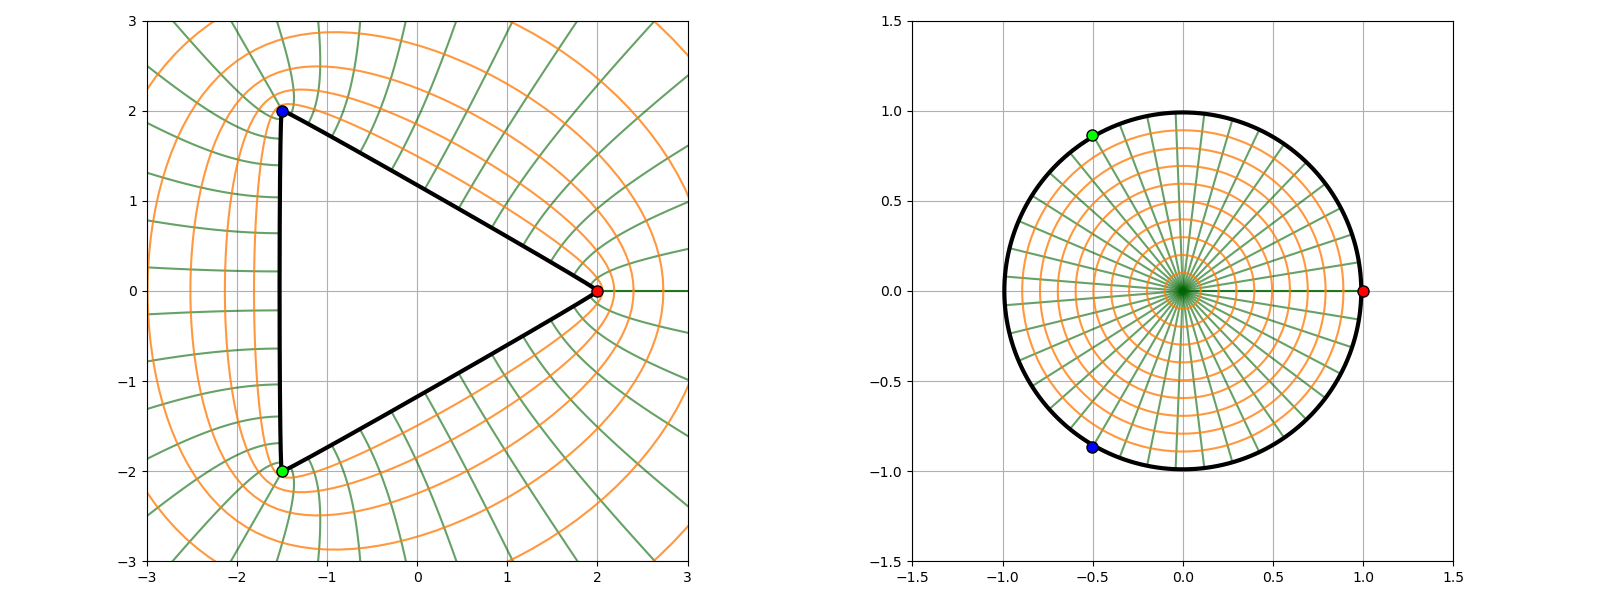
\includegraphics[width=0.9\textwidth]{papers/elektro/grafik/SC_trafo_triag.png}
	\caption{Schwarz-CHristoffel transfomriertes Polygon auf das innere des Einheitskreises}
	\label{elektro:figure:SC_triag_trafo}
\end{figure}

Auf der Abbilung \ref{elektro:figure:SC_triag_trafo} ist zu sehen wie die Feldlinien auf der Oberfläche des Dreiecks senkrecht aufkommen und sich im Raum ausbreiten und dabei auch die Potentiallinen immer senkrecht kreuzen.
Es sind auch die Prevertices auf dem Einheitskreis eingezeichnet die die Punkte markieren die exakt auf die Ecken des Dreiecks transfomiert werden, die farben zeigen welcher punkt auf welche Ecke transformiert wird. 
Dabei fällt auf, dass die Prevertices nicht intuitiv in der selben Richtung wie die Ecken des Dreiecks angeordnet sind, sondern in entgegengesetzten richtungen. 
Die ist auf eine Regel zurpckzuführen die besagt dass die Fläche die bearbeitet wird, im matematischen sinne, immer auf der linken Seite der Kurve liegen muss.
Dies kann so vorgestellt werdem: wenn die laufvariabel des Integrals sich auf der Kurve fortbewegt muss die Fläche die bearbeitet wird immer auf der linken Seite liegen.
Die Verlaufsrichtuung wird also immer so gewählt, dass dies Wahr ist.
Mit einem krleinen Gedanklichen experiment kann nun festgestellt werden dass die Verlaufsrichtung auf dem dreieck im Uhrzeigersinn sein muss und beim Einheitskreis gegen den Uhhrzeigersinn.


Als etwas komplexere Geometrie mit Mehreren Ecken darunter auch welche die einen grösseren Innewinkel als $180^{\circ}$ haben, wird ein Hufeisenförmiges Polygon gezeigt.
\begin{figure}
	\centering
	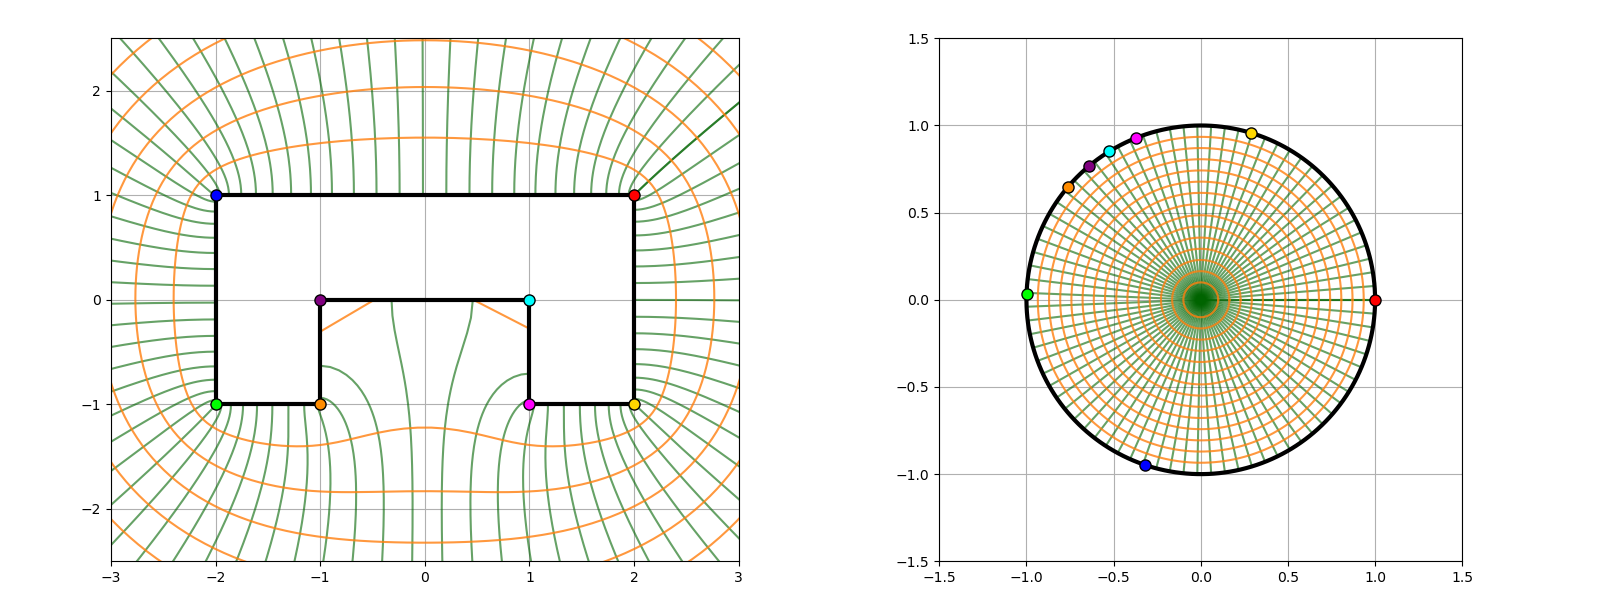
\includegraphics[width=0.9\linewidth]{papers/elektro/grafik/SC_trafo_huf.png}
	\caption{Schwarz-CHristoffel transfomriertes Polygon auf das innere des Einheitskreises}
	\label{elektro:figure:SC_huf_trafo}
\end{figure}

In den Beiden bereits besprochenne Beispielen ist das folgende auch schon zu sehen aber hier kommt noch ein etwas anschaulicheres Beispie, in Abbildung \ref{elektro:figure:SC_star_trafo} sind drei verschiedene Winkel zu finden, die alle eine andere konzentration an Feldlinen aufweisen die senkrecht dort wufkomen.
Bei spitzen winkkeln ist zu sehen das die Feldlinen näher beieinander sind und bei den stumpferen oder sogar überstumpfen Winkeln ist zu sehen dass die Feldlinen weiter auseinander liegen.
Dies ist auf die Ladungsverteilung zurückzuführen die sich auf dem Objekt verteilt.
Bei spitzeren winkeln hat es weniger platz zwischen den ebieden Kanten und LAdungsträger drücken die vor ihnen liegenden Ladungsträger näher zusammen, was zu einer höheren Ladungsdichte an den spitzen führt.
Bei den stumpferen Winkeln ist es genau umgekehrt, dort hat es mehr Platz und die Ladungsträger können sich weiter auseinander verteilen, da dies sowieso das ist was ladungsträger mit gleicher polarität am liebsten tun. 
Genau wie die E-Feldlinen die sich gegenseitig abstossen und sich so weit wie möglich voneinander entfernen.

\begin{figure}
	\centering
	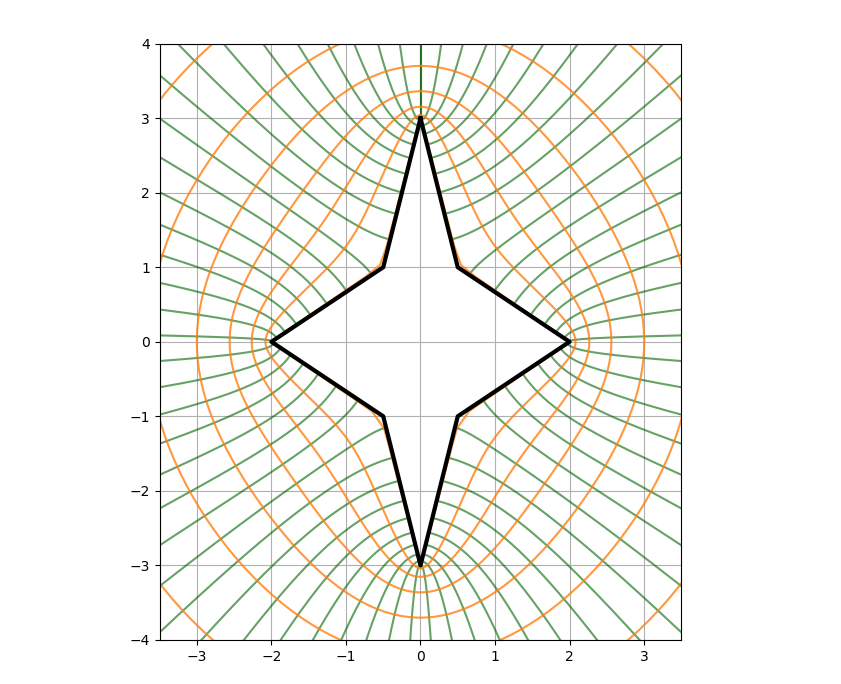
\includegraphics[width=0.9\linewidth]{papers/elektro/grafik/SC_trafo_star.png}
	\caption{Sternförmige Kontour mit verschiedenen Innenwinkeln}
	\label{elektro:figure:SC_star_trafo}
\end{figure}

Diese Spitzeneffekte sind nicht auf die Elektrostatik beschränkt sondern kommen in allen Bereichen der Physik vor.
In der Mechanik ist es das gleiche Prinzip, dass sich Kräfte an den Spitzen von Objekten konzentrieren und dort zu einer höheren Belastung führen.
In Abbildung \ref{elektro:figure:mech_triag} ist ein Beispiel zu sehen wie sich die Kräfte an den Spitzen eines Dreiecks konzentrieren.

\begin{figure}
	\centering
	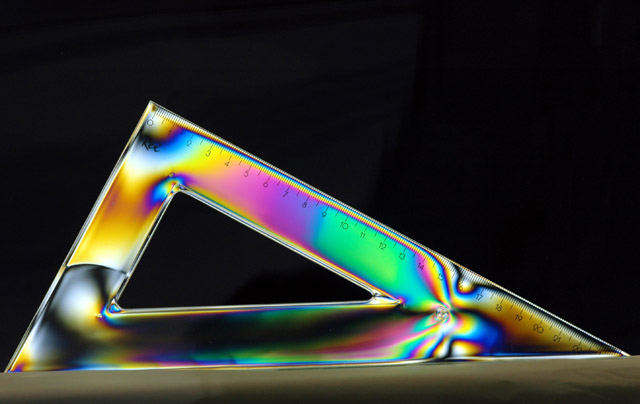
\includegraphics[width=0.9\linewidth]{papers/elektro/grafik/mech_triag.png}
	\caption{Kraftkonzentration an den Spitzen eines Dreiecks}
	\cite[Bild Quelle]{elektro:mech_triag}
	\label{elektro:figure:mech_triag}
\end{figure}

%\input{papers/elektro/00_grafiken.tex}

\printbibliography[heading=subbibliography]
\end{refsection}

%Vektorfelder einheitlich als \vec{E} schreiben
